% MA211 - Lecture 06
\documentclass[pdftex, xcolor=pdftex, dvipsnames,handout]{beamer}

\usetheme{MA211}
\usepackage{thumbpdf}
\usepackage{wasysym}
%\usepackage{ucs}
\usepackage[utf8]{inputenc}
\usepackage{pgf,pgfarrows,pgfnodes,pgfautomata,pgfheaps,pgfshade}
\usepackage{verbatim}

\usepackage{eurosym}
\usepackage{euler}

\usepackage{calc}               % Simple computations with LaTeX variables
%\usepackage[hang]{caption2}     % Improved captions

\usepackage{graphicx}           % Standard graphics package

\usepackage{amsmath, amsthm, amssymb}


\newcommand{\fquad}{\mbox{\qquad}}
\newcommand{\bull}{$\bullet$ }

\newcommand {\I} {\mathcal I}
\newcommand {\calI} {\mathcal I}
\def\disint{\displaystyle\int}

\DeclareMathOperator{\D}{d}
\newcommand{\dydx}{\frac{\D y}{\D x}}

%\definecolor{gray}{rgb}{0.69, 0.69, 0.69} \newcommand{\gray}[1]{\textcolor{gray}{#1}}
\definecolor{dogreen}{rgb}{0.33, 0.42, 0.18} \newcommand{\dogreen}[1]{\textcolor{dogreen}{#1}}
\definecolor{maroon}{rgb}{.5,0.2,0.2}\newcommand{\maroon}[1]{\textcolor{maroon}{#1}}
\definecolor{greena}{rgb}{.1,0.581,0.1}\newcommand{\greena}[1]{\textcolor{greena}{#1}}

\definecolor{blue4}{rgb}{0,0,.545}
\newcommand{\Blue}[1]{\textcolor{blue}{#1}}
\newcommand{\Red}[1]{\textcolor{red}{#1}}
\definecolor{pink}{rgb}{1.,0.75,0.8}
\definecolor{darkred}{rgb}{0.5,0.0,0.0}
\definecolor{darkgreen}{rgb}{0,0.3,0.3}
\definecolor{purple}{rgb}{0,0.3,0.3}
\definecolor{darkblue}{rgb}{0.0, 0.0, .5}
\definecolor{dpurple}{rgb}{.3,.0,.3}
\newcommand{\Green}[1]{\textcolor{darkgreen}{#1}}
\newcommand{\DRed}[1]{\textcolor{darkred}{#1}}
\newcommand{\DBlue}[1]{\textcolor{darkblue}{#1}}
\newcommand{\Purple}[1]{\textcolor{dpurple}{#1}}
\newcommand{\Emph}[1]{\textcolor{darkred}{\textbf{\it #1}}}
\newcommand{\remph}[1]{\textcolor{darkred}{\textbf{\emph{#1}}}}
\newcommand{\bemph}[1]{\textcolor{darkblue}{\textbf{\emph{#1}}}}
\newcommand{\gemph}[1]{\textcolor{darkgreen}{\textbf{\emph{#1}}}}
\newcommand{\Bf}[1]{\textcolor{darkblue}{\textbf{#1}}}
\newcommand{\Gf}[1]{\textcolor{darkgreen}{\textbf{#1}}}
\newcommand{\Rf}[1]{\textcolor{red}{\textbf{#1}}}
\newcommand{\Rmf}[1]{\textcolor{red}{\mathbf{#1}}}

\newcommand{\Conj}[1]{\overline{#1}}

\newcommand{\code}[1]{\textcolor{darkblue}{\texttt{\textbf{#1}}}}
\newcommand{\icode}[1]{{\blue\texttt{\textbf{\emph{#1}}}}}
\newcommand{\gcode}[1]{{\Green{\texttt{\textbf{\emph{#1}}}}}}
\newcommand{\out}[1]{\texttt{\emph{\textbf{\Green{#1}}}}}





\newenvironment{vminipage}%
{\begin{Sbox}\begin{minipage}\begin{small}\begin{verbatim}}%
{\end{verbatim}\end{small}\end{minipage}\end{Sbox}\fbox{\TheSbox}}

\newenvironment{nminipage}%
{\begin{Sbox}\begin{minipage}}%
{\end{minipage}\end{Sbox}\fbox{\TheSbox}}


\let\Arg\relax\DeclareMathOperator{\Arg}{\mathtt{Arg}}
\let\Arg\relax\DeclareMathOperator{\e}{\mathtt{e}}

\newcommand {\AND} {\wedge}
\newcommand {\OR} {\vee}
\newcommand {\NOT} {\neg}
\newcommand {\IMPLIES} {\rightarrow}
%\newcommand {\IFF} {\leftrightarrow}
\renewcommand {\iff} {\Leftrightarrow}
\newcommand {\NAND} {\uparrow}
\newcommand {\NOR} {\downarrow}
\newcommand {\XOR} {\otimes}

\newenvironment{citemize}% Colour items
{\begin{description}}%
{\end{description}}

\newcommand {\maroonitem}{\item[\maroon{$\bullet$}]}

\newcommand {\gitem} {\item {\includegraphics[width=.4cm,angle=-10]{img/green-bullet-on-white.ps}}}
\newcommand {\ritem} {\item {\includegraphics[width=.4cm,angle=-10]{img/red-bullet-on-white.ps}}}
\newcommand {\yitem} {\item {\includegraphics[width=.4cm,angle=-10]{img/yellow-bullet-on-white.ps}}}
\newcommand {\bitem} {\item {\includegraphics[width=.4cm,angle=-10]{img/blue-bullet-on-white.ps}}}

\newcommand {\greenitem} {\item {\includegraphics[width=.4cm,angle=-10]{img/green-bullet-on-white.ps}}}
\newcommand {\reditem} {\item {\includegraphics[width=.4cm,angle=-10]{img/red-bullet-on-white.ps}}}
\newcommand {\yellowitem} {\item {\includegraphics[width=.4cm,angle=-10]{img/yellow-bullet-on-white.ps}}}
\newcommand {\blueitem} {\item {\includegraphics[width=.4cm,angle=-10]{img/blue-bullet-on-white.ps}}}

\newcommand {\eq}[1]%
  {$\DBlue{#1}$}
\newcommand {\eqd}[1]%
  {$\displaystyle\DBlue{#1}$}
%\newcommand{\eq}[1]{\boldmath \DBlue{$#1$}}


\newcommand {\csf}{\centerslidesfalse}
\newcommand {\cst}{\centerslidestrue}

\newcommand {\vecii}[2] {   \big(\begin{smallmatrix} #1 \\ #2 \end{smallmatrix}\big)}
\newcommand{\atwo}[2]{\left(\!\!\begin{array}{c} #1 \\ #2 \end{array}\!\!\right)}


\newcommand{\C}{\mathbb{C}}
\newcommand{\Q}{\mathbb{Q}}
\newcommand{\R}{\mathbb{R}}
\newcommand{\N}{\mathbb{N}}
\newcommand{\Z}{\protect\mathbb{Z}}  % protect for index.
\newcommand {\Rs}{ \mathbb{R}}
\newcommand {\Cs}{ \mathbb{C}}
\newcommand {\Rnn}{ \mathbb{R}^{n \times n}}
\newcommand {\Rn}{ \mathbb{R}^{n}}


\newcommand{\mblock}{%
\setbeamercolor*{block title}{bg=maroon,fg=white}
\setbeamercolor*{block body}{bg=white,fg=maroon}
}%

\newcommand{\bblock}{%
\setbeamercolor*{block title}{bg=Steel,fg=white}
\setbeamercolor*{block body}{bg=Mylightgray,fg=Steel}
}%

\newcommand{\gblock}{%
\setbeamercolor*{block title}{bg=Green,fg=white}
\setbeamercolor*{block body}{bg=Mylightgray,fg=darkgreen}
}%


\newcommand{\rblock}{%
\setbeamercolor*{block title}{bg=Red,fg=white}
\setbeamercolor*{block body}{bg=white,fg=Black}
}%


\newcommand{\TakeNotes}{
\includegraphics[width=2cm]{TakeNote}}




\def\eps{\varepsilon}
\newcommand {\del}[2]{ {\frac{\partial #1}{\partial #2}}}
\newcommand {\x}[1]{x^{[#1]}}
\newcommand {\delx}{ {\frac{\partial}{\partial x}}}
\newcommand {\delt}{ {\frac{\partial}{\partial t}}}
\newcommand {\dely}{ {\frac{\partial}{\partial y}}}
\newcommand {\ith}{{(i)}}
\renewcommand {\vec}[1]{ {\boldsymbol{#1}}}
\newcommand {\Oh} {\mathcal O}
\newcommand {\Err} {\mathcal E}
%\newcommand {\th} {\mathrm{th}}
\DeclareMathOperator{\fl}{fl}
\DeclareMathOperator{\sign}{sign}
\DeclareMathOperator{\Cond}{Cond} 
\DeclareMathOperator{\cond}{cond}
\DeclareMathOperator{\diag}{diag} 
\DeclareMathOperator{\sym}{sym} 
\DeclareMathOperator{\Trace}{Trace}
\DeclareMathOperator{\E}{e}

\newcommand {\Rsym}{{ \mathbb{R}^{n \times n}_\mathrm{sym}}}

\parskip .25cm


\theoremstyle{definition}
\newtheorem{exercise}{Exercise}[section]
\newtheorem{method}{Method}[section]



\subtitle{MA211}
\title{Lecture 6: Antiderivatives and Integrals}

\author{Dr Niall Madden}

\date{\Large Wed 24 September 2008}


\begin{document}


\frame{

\begin{block}{}
\begin{center}
{\large \insertsubtitle}

\vspace{.1cm}

\begin{Large}
\textbf{\inserttitle}
\end{Large}

\vspace{.15cm}

% {\footnotesize \insertauthor}

\vspace{.3cm}

{ {\insertdate}}
\end{center}
\end{block}


\vspace{-0.25cm}
\begin{center}
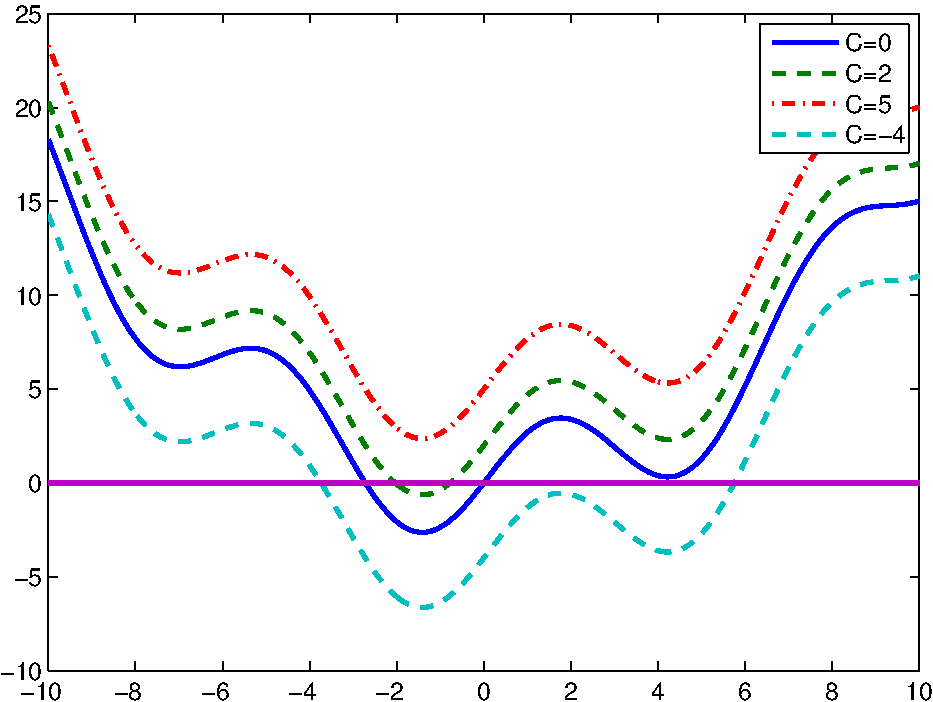
\includegraphics[height=4cm]{images/Fig4}

\end{center}
}





\frame{
\begin{center}
{\Large \Bf{Blackboard}}
\end{center}

From \alert{today} (24/09/08)  I won't be updating the pages at
\code{http://www.maths.nuigalway.ie/MA211/} 

If you are registered for MA211, you should be able to
access all course material through 
\href{http://blackboard.nuigalway.ie}{\code{http://blackboard.nuigalway.ie}}

If for some reason you  can't, then send me an email.


}

\frame{

\begin{center}
{\Large \Bf{Problem Set 1}}
\end{center}

\begin{block}{}
{\large \alert{Problem Set 1}} is available for down-load.


Write out,  clearly  and carefully, solutions to the selected
exercises and submit them by 11am, Monday Oct 6th.

~

However, you should attempt \Bf{all} exercises. Some of them may
feature on the final exam.
\end{block}

\pause
Tutorials take place
\begin{itemize}

\item Tuesday, 3pm, AC202

\item Wednesday, 5pm, QA003 (Physiology lecture room)


\end{itemize}

}


\frame{

\frametitle{In today's class...}


\begin{block}{}
\tableofcontents
\end{block}
}




\section{Antiderivatives}
\frame{

\code{See Stewart's \Emph{Calculus} 5.3}

On Monday we considered problems of the form: \Emph{given a function
  \eq{f} find it's derivative}. That is, find \eq{g} such that
\eqd{g(x) = \frac{d}{dx}f(x)}.


However, much of this course is related to the \emph{inverse} of this
problem: \emph{given a function
  \eq{f} find it's \Bf{antiderivative}}


\begin{definition}[Antiderivative]
Given a function \eq{f} in an interval \eq{I}, the function \eq{F} is
\Emph{an}  \Bf{antiderivative} of \eq{f} on \eq{I} if 
\[
F'(t) = f(t) \quad \text{ for all } x \in I.
\]
\end{definition}

}

\frame{

\begin{example}

\begin{itemize}[<+->]
\item \eq{F(t)=t} is an antiderivative of \eq{f(x)=1}.

~

~


\item \eq{F(t)=\frac{1}{2}t^2} is an  antiderivative of \eq{f(t)=t}.

~

~

\item \eq{F(t) = -cos(t)} is an antiderivative of \eq{f(t)=\sin(t)}.

~

\end{itemize}

\end{example}

\vspace{2cm}

}

\subsection{Indefinate Integrals}
\frame{

Note that \eq{F(t)=-1/t} is an antiderivative of \eq{f(t)=1/t^2}
(\emph{on any interval that excludes \eq{t=0}}).

%\pause

~

But so too is  \eq{F(t)= 5 -1/t} and \eq{F(t) = -1/t -3.1415} and,
indeed, any function of the form 
\eq{F(t) = -1/t + C} for some constant \eq{t}.

%\pause

~

When we write down the antiderivative of \eq{f} and include the
constant \eq{C} we usually call it the \Bf{General Antiderivative} of
\eq{f} or, more commonly, the \Emph{The Indefinate Integral}.


}


\frame{

\begin{definition}[Indefinite Integral]
The \Bf{Indefinite Integral} of \eq{f(t)} on the interval \eq{I} is
\[
\int f(t) dt = F(t) + C \quad \text{ for } t \in I,
\]
where \eq{F'(t) = f(t)} for all \eq{t} in \eq{I}.
\end{definition}
We call \eq{C} the \Emph{constant of integration}.




\pause

(\emph{Next week we'll do \Bf{definate integrals}, which have limits of integration:
\eqd{\int_a^b f(x) dx}}).

}

\subsection{Fundamental Examples}
\frame{

%\Header{Examples}

\begin{enumerate}[<+->]

\item \eqd{\int 1 \ dx = }

~

~

\item \eqd{\int x \ dx = }

~

~


\item \eqd{\int x^2 dx =}

~

~

\item \eqd{\int x^n dx =}

~

~


\end{enumerate}
}


\frame{

\begin{enumerate}\setcounter{enumi}{4}


\item \eqd{\int \sin(x)  dx =}

~

~


\item \eqd{\int \cos(x) dx =}
~

~


\end{enumerate}

}

\subsection{The Mathematical Tables}

\frame{

It is neither important or necessary to memorise the antiderivatives
of even reasonably common functions. However, you should be able to
look them up on pages 41 and 42 of the Mathematical Tables.

Having p9 is also handy.

}

\frame{
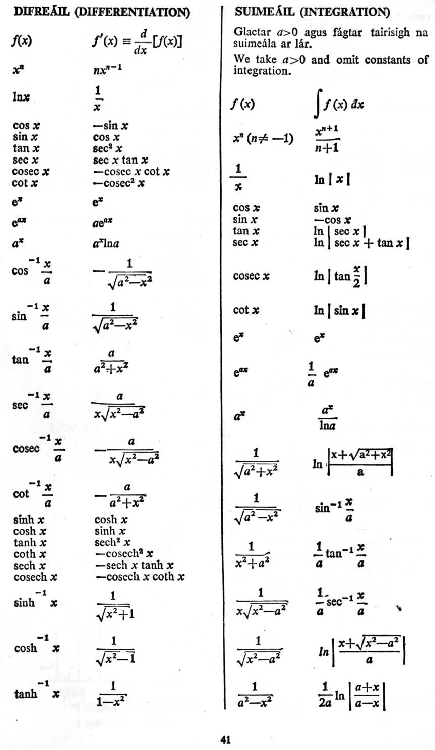
\includegraphics[angle=90, width=11.25cm]{images/p41}
}
\frame{
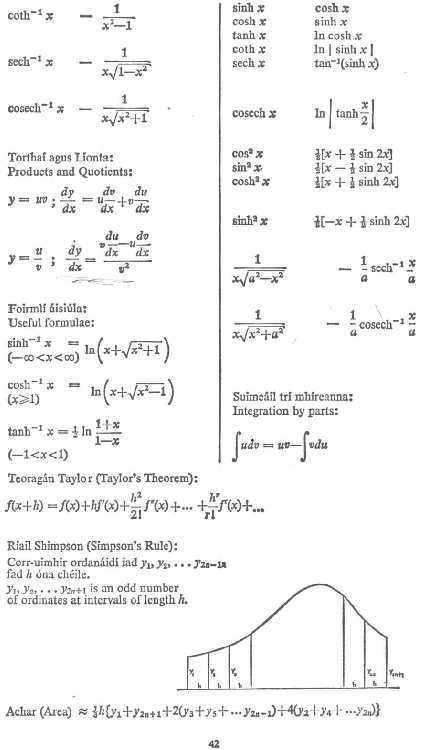
\includegraphics[angle=90, width=11.25cm]{images/p42}
}
\frame{
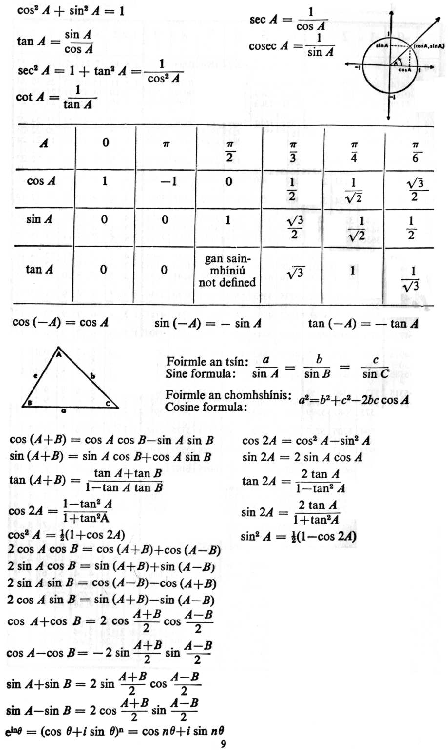
\includegraphics[angle=90, width=11.25cm]{images/p9}
}

\subsection{More examples}

\frame{

\begin{example}
\begin{enumerate}[<+->]

\item  \eqd{\int \big( x^3 -5x^2 +7\big) dx =}

\vspace{1cm}

\item  \eqd{\int  x^{-3}  dx =}


\vspace{1cm}

\end{enumerate}
\end{example}

}

\frame{

\begin{example}
\begin{enumerate}[<+->]
\item[3.]  \eqd{\int  x^{-n}  dx =}

\vspace{1cm}

\item[4.]  \eqd{\int  x^{-1}  dx =}

\vspace{1cm}

\item[5.]  \eqd{\int  \frac{\sin(t)}{\tan(t)}  dt =}

\vspace{1cm}

\end{enumerate}
\alert{Don't forget the constant of integration!}

\end{example}
}

\frame{

\begin{exercise}[Q6.1]
\begin{enumerate}[(i)]
\item $ 6t^2 -1$,
\item \eqd{ \frac{x+3}{x^{3/2}}}
\item \eq{\int 6 dx} 
\item \eqd{\int x^{-2} dx}
\item \eqd{\int\big(x^2 + \cos(x)\big) dx}
\item \eq{\int \cos (t) \tan (t) dt}
\item \eqd{\int (A + Bx + Cx^2) dx}
\item \eqd{\int \cos(3x) dx}
\end{enumerate}

\alert{Don't forget the constant of integration!}
\end{exercise}
}


\section{Differential equations}
\frame{

When we see a problem like:
\begin{block}{}
\begin{center}
Evaluate \eqd{\int  3t^2-1  dt } 
\end{center}
\end{block}
we can think of it as 
\begin{block}{}
\begin{center}
Find a function whose derivative (with respect to \eq{t}) is \eqd{3t^2 -1}.
\end{center} 
\end{block}
\pause
Another equivalent way of asking the same question is:
\begin{block}{}
\begin{center}
Find a function \eq{f} that solves the equation  \eqd{f'(t) =  3t^2 -1}.
\end{center} 
\end{block}

\pause
This is an example of a simple \Emph{Differential Equation (DE)}, and we'll
study much more of these as  go through the course.

}

\frame{

Our 1st Differential Equation is:
\begin{example}[1]
\begin{center}
Find a function \eq{f} that solves the equation  \eqd{f'(t) =  3t^2 -1}.
\end{center} 
\end{example}
and its solution is of the form
\[ f(t) = t^3 -t +C \]
for an \Emph{arbitrary} constant \eq{C}. 

\pause
\begin{definition}[General Solution]
The \Bf{general solution} of a differential equation is one that includes
one or more arbitrary constants corresponding to constants of
integration.
\end{definition}

}

\frame{

\begin{example}[2]
Find the general solution to the differential equation 
\[ f''(x)=x.\]
\end{example}

\vspace{4cm}

}

\frame{

\begin{example}[3]
Show that the function
\[ f(x) = C_1x^3 + C_2/x\]
is a solution to the differential equation
\[ x^2 f''(x) - xf'(x) -3f(x) = 0.\]
\end{example}

\vspace{4cm}

}


\frame{

\begin{exercise}[Q6.2]
\begin{enumerate}[(i)] 
\item Show that, for any constants \eq{C_1} and \eq{C_2}, 
\[ y(x) = C_1x^2 + C_2x^{-2} \] 
is a solution to the differential
equation
\[ x^3y'''(x) + 6x^2 y''(x) = 12 y(x). \]


\item Write down a 2nd order differential equation that has $f(x)=x^2
  -x$ as a solution.
\end{enumerate}
\end{exercise}

}

\frame{

\begin{example}[4]
Write down the \Bf{general solution} to the following differential equation:
\[ y'(x) = x/3 + 3\cos(x)\]
\end{example}

}

\frame{
\begin{center}
{\eqd{\frac{x^2}{6} + 3 \sin(x) + C}}


\only<4>{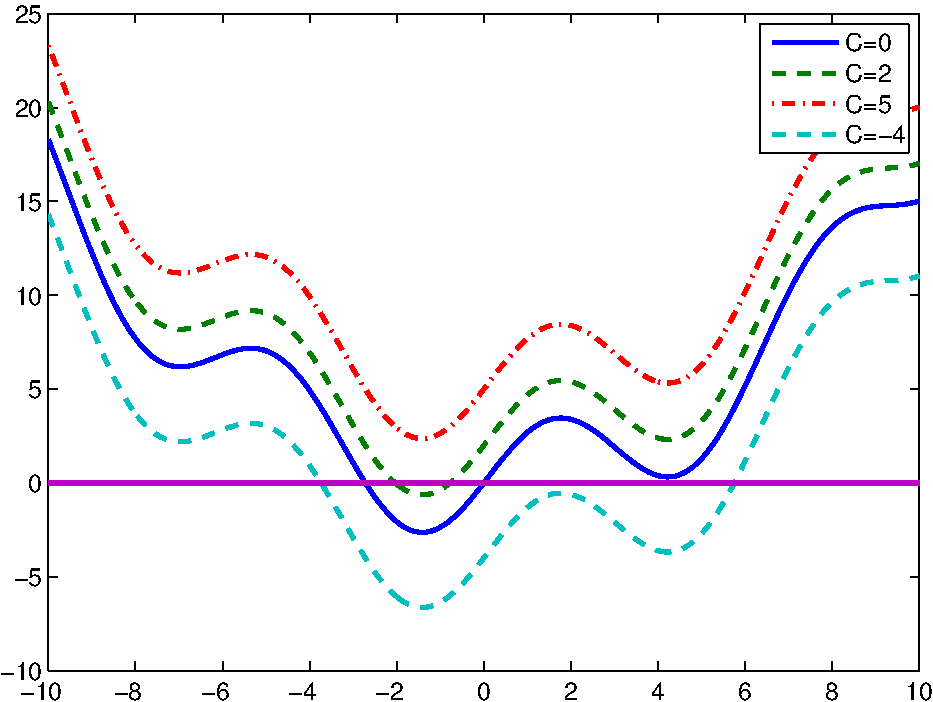
\includegraphics[width=9cm]{images/Fig4}}
\only<1>{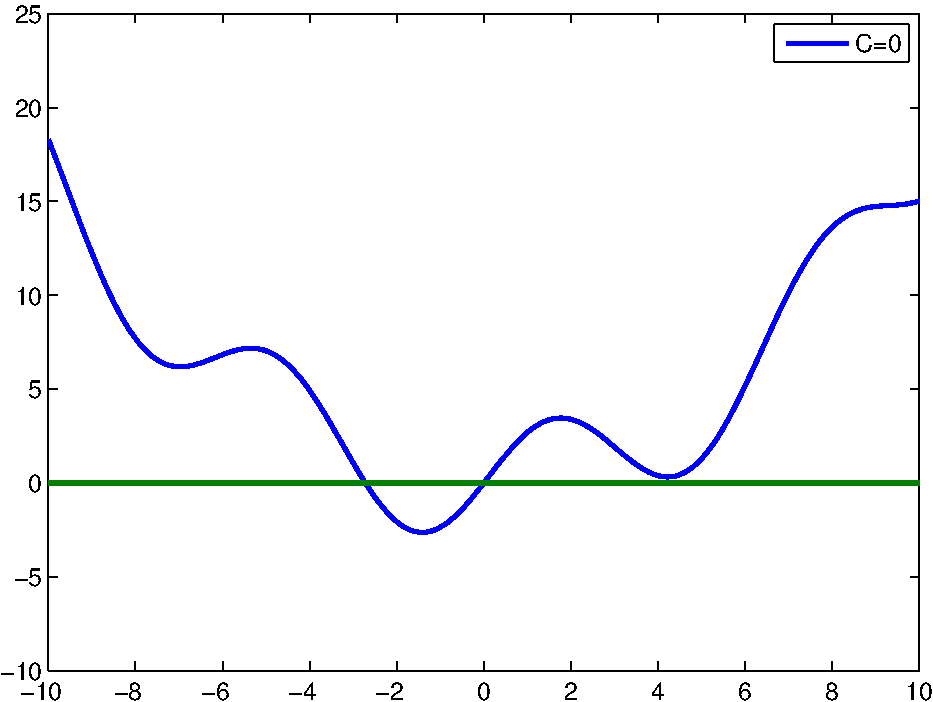
\includegraphics[width=9cm]{images/Fig1}}
\only<2>{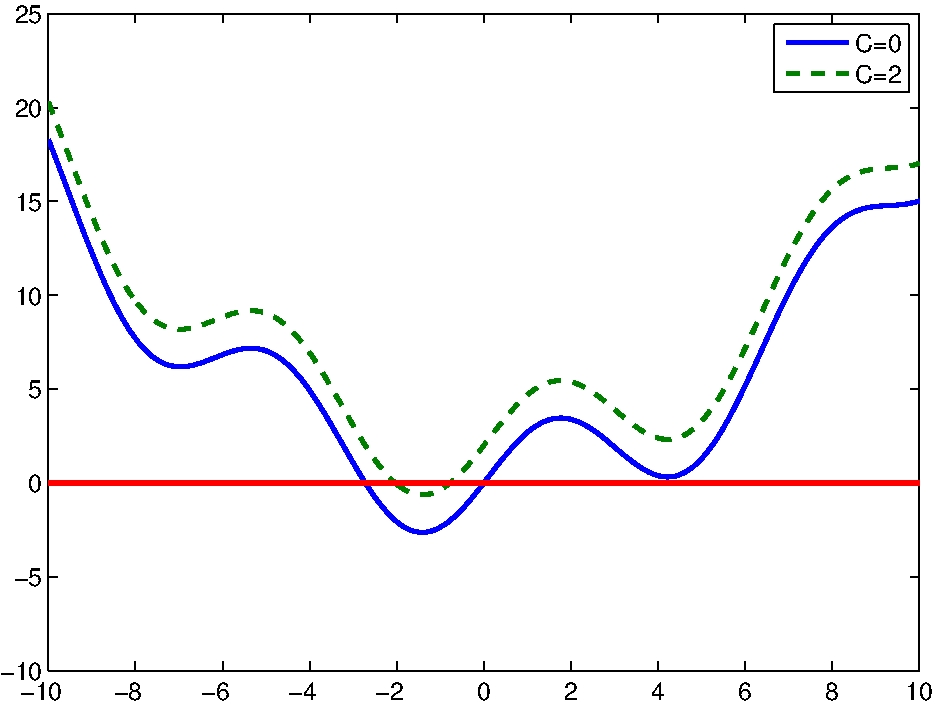
\includegraphics[width=9cm]{images/Fig2}}
\only<3>{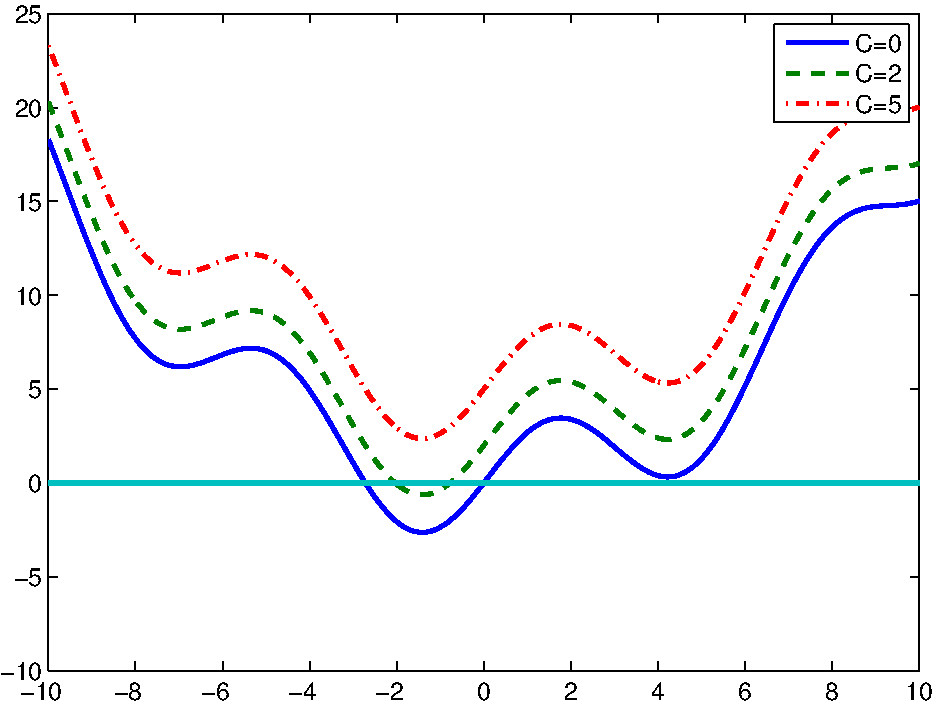
\includegraphics[width=9cm]{images/Fig3}}
\end{center}

}

\section{General V Particular Solutions}


\frame{

The following is an example of a simple differential equation:
\begin{block}{}
\Bf{Q:} If you travel east at a constant speed of 90km/hr for 1 hour, where are you?

\Emph{A:} 90km east of where we started!\\
This is the \Emph{general solution}.
\end{block}

~

\pause
An alternative problem is:
\begin{block}{}
\Bf{Q:} If you travel east \Emph{from Galway} at a constant speed of 90km/hr for 1 hour, where are you?

\Emph{A:} Athlone.\\
This is a \Emph{particular solution}: the arbitrary constant is specified.
\end{block}

}




\section{Particular Solutions}
\frame{
\begin{example}[5]
Find the solution to the differential equation
\[ y'(x)  = \frac{x}{3} + 3\cos(x),\]
given that \eqd{y(0)=2.}
\end{example}

%The general solution is 
%\[ y(x) = \frac{x^2}{6} + 3 \sin(x) + C.\]
%If \eq{y(0)=2}, then
%\[
%\frac{\alert{0}^2}{6} + 3 \sin(\alert{0}) + C = C= 2.\]
\vspace{4cm}



%So the particular solution is 
%\eqd{y(x) = \frac{x^2}{6} + 3 \sin(x) + 2.}

}

\frame{

\begin{exercise}[Q6.3]
Find  solutions to the following  differential equations. If possible,
gave a particular solution, otherwise, give the general solution.

\begin{enumerate}[(i)]
\item $y'(t) = x-2$
~

\item  \eq{f'(x) = x^{-2} - x^{-3}},  subject to \eq{f(-1)=0}.
~

\item $y''(x) = x^3-1$,  given that $y'(0)=0, y(0)=8$.
\end{enumerate}

\end{exercise}
}




\end{document}
